\documentclass[11pt]{article}
\usepackage[margin=1in]{geometry}
\usepackage{amsmath,amssymb,amsthm}
\usepackage{graphicx}
\usepackage{float}
\usepackage[hidelinks]{hyperref}
\usepackage{microtype}
\setlength{\emergencystretch}{2em}
\setlength{\intextsep}{6pt}
\setlength{\abovecaptionskip}{4pt}
\graphicspath{{figures/}}

\DeclareMathOperator{\tr}{trace}
\DeclareMathOperator{\Var}{Var}
\DeclareMathOperator{\Cov}{Cov}
\newcommand{\E}{\mathbb{E}}
\newcommand{\R}{\mathbb{R}}
\newcommand{\mat}[1]{\begin{bmatrix}#1\end{bmatrix}}

\title{CSE 242 -- Assignment 1}
\author{Yi Zhong \\ \texttt{yzhong76@ucsc.edu}}
\date{Fall 2026}

\begin{document}
\maketitle

%======================================================================
\section{Linear Algebra}

\subsection{Q1}
$A=\mat{3&4\\2&1}$, $B=\mat{1&2\\0&-1}$.
\begin{align*}
AB &= \mat{3\cdot1+4\cdot0 & 3\cdot2+4\cdot(-1)\\ 2\cdot1+1\cdot0 & 2\cdot2+1\cdot(-1)}
    = \mat{3&2\\2&3}\\[4pt]
BA &= \mat{1\cdot3+2\cdot2 & 1\cdot4+2\cdot1\\ 0\cdot3+(-1)\cdot2 & 0\cdot4+(-1)\cdot1}
    = \mat{7&6\\-2&-1}\\[4pt]
(A+B)^T &= \mat{4&6\\2&0}^T = \mat{4&2\\6&0}\\[4pt]
AB^T &= \mat{3&4\\2&1}\mat{1&0\\2&-1}
     = \mat{3\cdot1+4\cdot2 & 3\cdot0+4\cdot(-1)\\ 2\cdot1+1\cdot2 & 2\cdot0+1\cdot(-1)}
     = \mat{11&-4\\4&-1}\\[4pt]
\tr(A) &= 3+1 = 4,\qquad
\tr(AB) = 3+3 = 6
\end{align*}

\subsection{Q2}
$M=\mat{2&-1\\-1&2}$.
\begin{gather*}
\det(M-\lambda I)=\det\mat{2-\lambda&-1\\-1&2-\lambda}
=(2-\lambda)^2-1=\lambda^2-4\lambda+3=(\lambda-1)(\lambda-3),\\
\det(M-\lambda I)=0\;\Rightarrow\;\lambda_1=1,\ \lambda_2=3 .
\end{gather*}
Eigenvectors $v=(v_1,v_2)^T$ solve $(M-\lambda I)v=0$:
\begin{align*}
\lambda_1=1:&\quad \mat{1&-1\\-1&1}\mat{v_1\\v_2}=0
\;\Rightarrow\; v_1=v_2 \;\Rightarrow\; v=\mat{1\\1}\\[2pt]
\lambda_2=3:&\quad \mat{-1&-1\\-1&-1}\mat{v_1\\v_2}=0
\;\Rightarrow\; v_1=-v_2 \;\Rightarrow\; v=\mat{1\\-1}
\end{align*}
Check $Mv=\lambda v$:
\[
M\mat{1\\1}=\mat{2-1\\-1+2}=\mat{1\\1}=1\cdot\mat{1\\1},\qquad
M\mat{1\\-1}=\mat{2+1\\-1-2}=\mat{3\\-3}=3\cdot\mat{1\\-1} .
\]

\subsection{Q3}
Let $A\in\R^{m\times n}$, $B\in\R^{n\times m}$. Then
\[
\tr(AB)=\sum_{i=1}^{m}(AB)_{ii}=\sum_{i=1}^{m}\sum_{j=1}^{n}A_{ij}B_{ji}
=\sum_{j=1}^{n}\sum_{i=1}^{m}B_{ji}A_{ij}
=\sum_{j=1}^{n}(BA)_{jj}=\tr(BA),
\]
where the third equality exchanges the order of the two finite sums.\qed

\subsection{Q4}
$C=\mat{4&7\\2&6}$, $\det C = 4\cdot6-7\cdot2 = 10\neq0$, so $C^{-1}$ exists.
To compute it, row-reduce the augmented matrix $[\,C\mid I\,]$ until the left
block becomes $I$; the right block is then $C^{-1}$ ($R_i$ denotes row $i$):
\begin{align*}
\left[\begin{array}{cc|cc}4&7&1&0\\2&6&0&1\end{array}\right]
&\xrightarrow{R_1\leftarrow R_1/4}
\left[\begin{array}{cc|cc}1&\tfrac74&\tfrac14&0\\2&6&0&1\end{array}\right]
\xrightarrow{R_2\leftarrow R_2-2R_1}
\left[\begin{array}{cc|cc}1&\tfrac74&\tfrac14&0\\0&\tfrac52&-\tfrac12&1\end{array}\right]\\[4pt]
&\xrightarrow{R_2\leftarrow \tfrac25 R_2}
\left[\begin{array}{cc|cc}1&\tfrac74&\tfrac14&0\\0&1&-\tfrac15&\tfrac25\end{array}\right]
\xrightarrow{R_1\leftarrow R_1-\tfrac74R_2}
\left[\begin{array}{cc|cc}1&0&\tfrac35&-\tfrac7{10}\\0&1&-\tfrac15&\tfrac25\end{array}\right]
\end{align*}
(last step: $\tfrac14-\tfrac74\cdot(-\tfrac15)=\tfrac14+\tfrac7{20}=\tfrac35$,
$0-\tfrac74\cdot\tfrac25=-\tfrac7{10}$). Hence
\[
C^{-1}=\mat{\tfrac35&-\tfrac7{10}\\[2pt]-\tfrac15&\tfrac25}=\mat{0.6&-0.7\\-0.2&0.4}.
\]

%======================================================================
\section{Probability, MLE and MAP}

\subsection{Q1}
$P(X=k)=c\,\dfrac{3^k}{k!}$, $k=0,1,2,\dots$

\noindent\textbf{(a)} The probabilities must sum to 1; with $\sum_{k\ge0}x^k/k!=e^x$,
\[
\sum_{k=0}^{\infty}c\,\frac{3^k}{k!}=c\,e^{3}=1
\;\Rightarrow\; c=e^{-3}.
\]
\noindent\textbf{(b)}
\begin{align*}
\E[X]&=\sum_{k=0}^{\infty}k\,e^{-3}\frac{3^k}{k!}
=3e^{-3}\sum_{k=1}^{\infty}\frac{3^{k-1}}{(k-1)!}=3e^{-3}e^{3}=3\\
\E[X(X-1)]&=\sum_{k=0}^{\infty}k(k-1)\,e^{-3}\frac{3^k}{k!}
=9e^{-3}\sum_{k=2}^{\infty}\frac{3^{k-2}}{(k-2)!}=9e^{-3}e^{3}=9\\
\E[X^2]&=\E[X(X-1)]+\E[X]=9+3=12\\
\Var(X)&=\E[X^2]-(\E[X])^2=12-9=3 \qquad\text{(by Q6)}
\end{align*}

\subsection{Q2}
$P(A)=0.5$, $P(B)=0.3$, $P(A\mid B)=0.6$.
\begin{align*}
\text{(a)}\quad P(A\cap B)&=P(A\mid B)\,P(B)=0.6\times0.3=0.18\\
\text{(b)}\quad P(B\mid A)&=\frac{P(A\cap B)}{P(A)}=\frac{0.18}{0.5}=0.36\\
\text{(c)}\quad P(A\cup B)&=P(A)+P(B)-P(A\cap B)=0.5+0.3-0.18=0.62
\end{align*}

\subsection{Q3}
Data H,\,H,\,T,\,H,\,T: 3 heads, 2 tails; each flip is Bernoulli($\theta$).

\noindent\textbf{(a)} Likelihood and log-likelihood:
\begin{gather*}
L(\theta)=\theta\cdot\theta\cdot(1-\theta)\cdot\theta\cdot(1-\theta)=\theta^{3}(1-\theta)^{2},\qquad
\ell(\theta)=\log L(\theta)=3\log\theta+2\log(1-\theta)\\
\ell'(\theta)=\frac{3}{\theta}-\frac{2}{1-\theta}=0
\;\Rightarrow\;3(1-\theta)=2\theta\;\Rightarrow\;\hat\theta_{\mathrm{MLE}}=\frac35
\end{gather*}
$\ell''(\theta)=-3/\theta^2-2/(1-\theta)^2<0$ and $L(0)=L(1)=0$, so this is
the maximum.

\noindent\textbf{(b)} Posterior $\propto$ likelihood $\times$ prior:
\begin{gather*}
P(\theta\mid\text{data})\propto L(\theta)P(\theta)=\theta^{3}(1-\theta)^{2}\cdot2\theta=2\theta^{4}(1-\theta)^{2}\\
\log P(\theta\mid\text{data})=4\log\theta+2\log(1-\theta)+\text{const}\\
\frac{d}{d\theta}:\;\frac{4}{\theta}-\frac{2}{1-\theta}=0
\;\Rightarrow\;4(1-\theta)=2\theta\;\Rightarrow\;\hat\theta_{\mathrm{MAP}}=\frac23
\end{gather*}
Second derivative $-4/\theta^2-2/(1-\theta)^2<0$ and the posterior is $0$ at
$\theta=0,1$, so this is the maximum.

\subsection{Q4}
For $x_1,\dots,x_n$ i.i.d.\ $\mathcal N(\mu,\sigma^2)$ the log-likelihood is
\[
\ell(\mu,\sigma^2)=\sum_{i=1}^{n}\log\frac{1}{\sqrt{2\pi\sigma^2}}
e^{-(x_i-\mu)^2/(2\sigma^2)}
=-\frac n2\log(2\pi\sigma^2)-\frac{1}{2\sigma^2}\sum_{i=1}^{n}(x_i-\mu)^2 .
\]
Setting the partial derivatives to zero (data $\{1,3,5,7\}$, $n=4$):
\begin{align*}
\frac{\partial\ell}{\partial\mu}&=\frac{1}{\sigma^2}\sum_{i=1}^{n}(x_i-\mu)=0
&&\Rightarrow\;\hat\mu=\frac1n\sum_{i=1}^{n}x_i=\frac{1+3+5+7}{4}=4\\
\frac{\partial\ell}{\partial\sigma^2}&=-\frac{n}{2\sigma^2}+\frac{1}{2\sigma^4}\sum_{i=1}^{n}(x_i-\mu)^2=0
&&\Rightarrow\;\hat\sigma^2=\frac1n\sum_{i=1}^{n}(x_i-\hat\mu)^2=\frac{(-3)^2+(-1)^2+1^2+3^2}{4}=5
\end{align*}

\subsection{Q5}
$x\mid\mu\sim\mathcal N(\mu,\sigma^2)$, $\sigma^2=4$; $\mu\sim\mathcal N(\mu_0,\tau^2)$,
$\mu_0=0,\ \tau^2=1$; $x=5$. Posterior $\propto$ likelihood $\times$ prior:
\begin{gather*}
\log P(\mu\mid x)=\log P(x\mid\mu)+\log P(\mu)+\text{const}
=-\frac{(x-\mu)^2}{2\sigma^2}-\frac{(\mu-\mu_0)^2}{2\tau^2}+\text{const}\\
=-\frac{(5-\mu)^2}{8}-\frac{\mu^2}{2}+\text{const}\\
\frac{d}{d\mu}:\;\frac{5-\mu}{4}-\mu=0\;\Rightarrow\;5-\mu=4\mu\;\Rightarrow\;\hat\mu_{\mathrm{MAP}}=1
\qquad\Big(\tfrac{d^2}{d\mu^2}=-\tfrac14-1<0\Big)
\end{gather*}

\subsection{Q6}\label{sec:varexp}
Let $\mu=\E[X]$. By linearity of expectation,
\begin{align*}
\Var(X)&=\E[(X-\mu)^2]=\E[X^2-2\mu X+\mu^2]
=\E[X^2]-2\mu\,\E[X]+\mu^2\\
&=\E[X^2]-2\mu^2+\mu^2=\E[X^2]-(\E[X])^2 .\qquad\qed
\end{align*}

%======================================================================
\section{Principal Component Analysis}

\subsection{Q1}\label{sec:proj}
Let $X\in\R^d$ be a random vector with mean $\mu=\E[X]$ and covariance
matrix $\Sigma=\E\big[(X-\mu)(X-\mu)^T\big]$, i.e.\ $\Sigma_{ij}=\Cov(X_i,X_j)$.
For a unit vector $u\in\R^d$ let $Y=u^TX$. Then $\E[Y]=u^T\E[X]=u^T\mu$, and
\begin{align*}
\Var(Y)&=\E\big[(u^TX-u^T\mu)^2\big]
=\E\big[(u^T(X-\mu))^2\big]\\
&=\E\big[u^T(X-\mu)(X-\mu)^Tu\big]
&&\text{(}(u^Tz)^2=u^Tzz^Tu\text{)}\\
&=u^T\,\E\big[(X-\mu)(X-\mu)^T\big]\,u
&&\text{($u$ constant, $\E$ linear)}\\
&=u^T\Sigma u .\qquad\qed
\end{align*}

\subsection{Q2}
$n=500$ samples drawn with NumPy (\texttt{multivariate\_normal}, seed 0)
from $\mathcal N(\mu,\Sigma)$ with
\[
\mu=\mat{2\\-1},\qquad \Sigma=\mat{3&1.2\\1.2&1},\qquad
\text{correlation }\rho=\frac{\Sigma_{12}}{\sqrt{\Sigma_{11}\Sigma_{22}}}=\frac{1.2}{\sqrt{3\cdot1}}\approx0.693 .
\]

\begin{figure}[H]
\centering
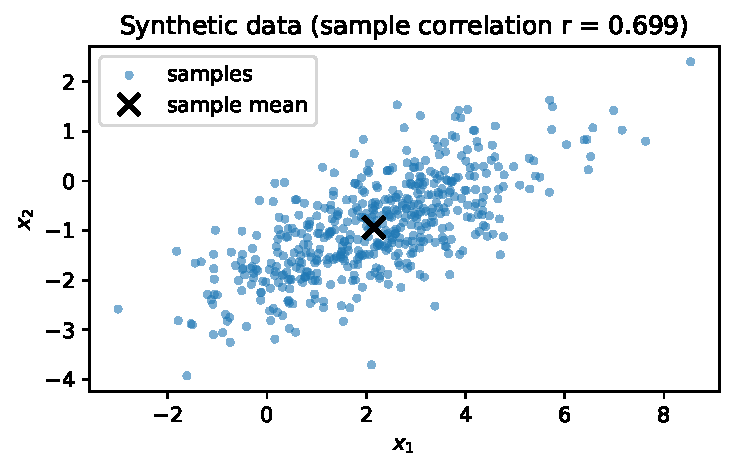
\includegraphics[width=0.45\textwidth]{data.pdf}
\caption{Synthetic samples and their sample mean.}
\label{fig:data}
\end{figure}

Sample mean, covariance and correlation:
$\bar x=\mat{2.152\\-0.935}$,
$\hat\Sigma=\mat{2.916&1.166\\1.166&0.953}$,
$r=0.699$.
The cloud is an ellipse tilted with positive slope, i.e.\ $x_1$ and $x_2$ are
positively correlated ($\Sigma_{12}>0$); it is wider along $x_1$ because
$\Var(x_1)=3>\Var(x_2)=1$. With $r\approx0.7$ the correlation is strong but
not perfect: the points scatter around the line rather than on it.

\subsection{Q3}
\begin{enumerate}
\item Centre: with $X$ the $n\times2$ data matrix, $\bar x=\frac1n\sum_i x_i$
  and $X_c=X-\mathbf 1\bar x^T$.
\item Covariance: $\hat\Sigma=\frac{1}{n-1}X_c^TX_c$ (sample version of
  $\E[(X-\mu)(X-\mu)^T]$).
\item Eigendecomposition: $\hat\Sigma=V\Lambda V^T$ with
  \texttt{np.linalg.eigh}, eigenvalues sorted descending.
\item By Section~\ref{sec:proj}, the variance of the data projected on a unit
  $u$ is $u^T\hat\Sigma u$; for an eigenvector $v_k$ it is
  $v_k^T\lambda_kv_k=\lambda_k$. So the columns of $V$ (ordered by $\lambda$)
  are the principal components, and $\lambda_k$ is the variance along each.
\end{enumerate}
\[
\hat\Sigma=\mat{2.916&1.166\\1.166&0.953},\qquad
\lambda_1=3.458,\ \lambda_2=0.411,\qquad
V=\mat{-0.907&0.422\\-0.422&-0.907}.
\]

\begin{figure}[H]
\centering
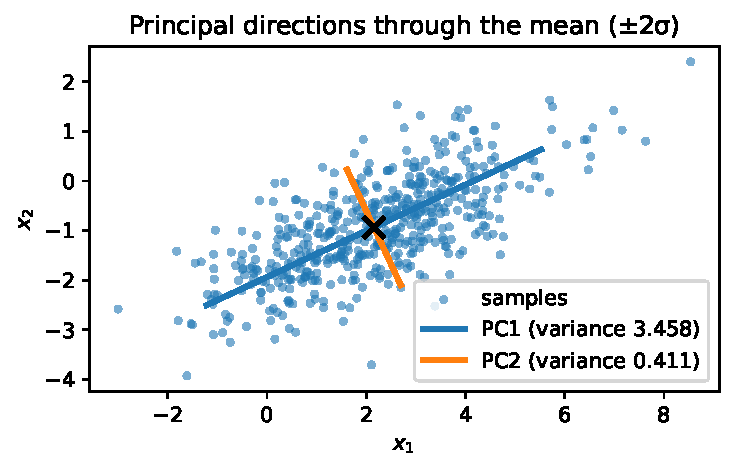
\includegraphics[width=0.45\textwidth]{pca.pdf}
\caption{Principal directions through the sample mean; each segment spans
$\pm2\sqrt{\lambda_k}$.}
\label{fig:pca}
\end{figure}

PC1 lies along the long axis of the ellipse, PC2 is orthogonal along the
short axis; the segment lengths $2\sqrt{\lambda_k}$ ($3.7$ vs $1.3$) match
the spread of the data in each direction.

\subsection{Q4}
Proportion of variance explained by component $k$:
\[
f_k=\frac{\lambda_k}{\lambda_1+\lambda_2}:\qquad
f_1=\frac{3.458}{3.869}=0.894,\qquad f_2=\frac{0.411}{3.869}=0.106 .
\]

\begin{figure}[H]
\centering
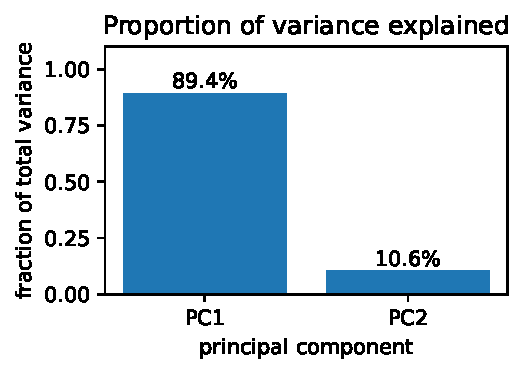
\includegraphics[width=0.3\textwidth]{explained_variance.pdf}
\caption{Proportion of variance explained by each component.}
\label{fig:var}
\end{figure}

PC1 alone explains $89.4\%$ of the variance, so projecting onto PC1 reduces
the data from 2 to 1 dimension while keeping $89.4\%$ of its variance. The
reduced data is more compact and easier to visualise, and the dropped
low-variance direction is often mostly noise. The trade-off: the $10.6\%$
along PC2 is lost, including any signal it carried, because PCA ranks
directions by variance, not by relevance to a task.

\end{document}
